\documentclass{article}
\usepackage{tikz}
\usetikzlibrary{shapes.gates.logic.US}
\usetikzlibrary{circuits.ee.IEC}

\usepackage[utf8]{inputenc}
\usepackage{amsmath}
\usepackage{amsfonts}
\usepackage{multicol}
\usepackage{amssymb}
\usepackage[framed]{matlab-prettifier}
\usepackage{graphicx}
\usepackage[margin=0.75in]{geometry}
\usepackage{enumerate}
\usepackage{circuitikz}


\title{Assignment 1 | FPGA Lab}
\author{EE22MTECH02005}
\date{January 2022}

\begin{document}


\maketitle

\section{Question 1}
Write the Boolean Expression for the result of the logic circuit as shown below:
 
    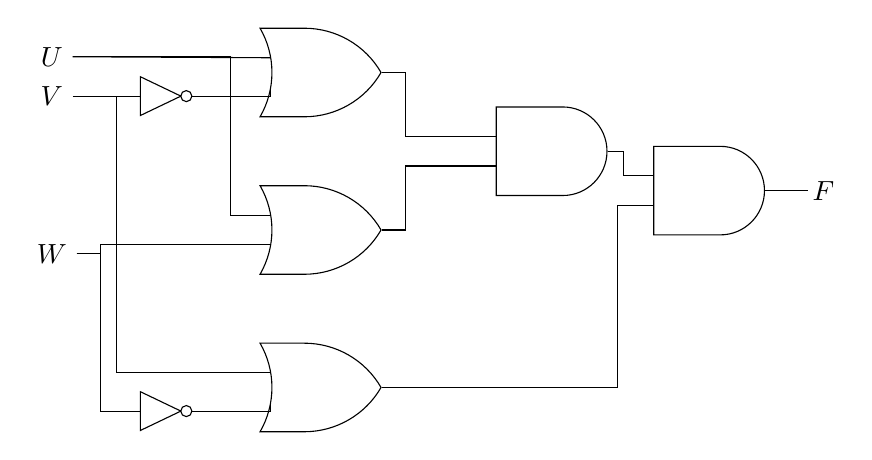
\begin{tikzpicture}[ circuit symbol wires]
    \node (x) at (-1.8,4.7) {$U$};
    \node (y) at (-1.8,2.2) {$W$};
    \node (z) at (-1.8,4.2) {$V$};
    \node[or gate US, minimum size=32pt, draw] at (1.5,0.5) (or1) {};
    \node[or gate US, minimum size=32pt, draw] at (1.5,2.5) (or2) {};
    \node[and gate US, minimum size=32pt, draw] at (4.5,3.5) (And21) {};
    \node[or gate US, minimum size=32pt, draw] at (1.5,4.5) (or3) {};
    \node[and gate US, minimum size=32pt, draw] at (6.5,3) (And22) {};
    \node[not gate US, minimum size=12pt, draw] at (-0.5,0.2) (not1) {};
    \node[not gate US, minimum size=12pt, draw] at (-0.5,4.2) (not2) {};
    \draw (y.east) - ++(right:3mm) |- (not1.input);
    \draw (y.east) - ++(right:3mm) |- (or2.input 2);
    \draw (x.east)-- (or3.input 1);
    \draw (x.east) - ++(right:2cm) |- (or2.input 1);
    \draw (z.east) - ++(right:5.5mm) |- (or1.input 1);
    \draw (z.east) - ++(right:3mm) -- (not2.input);
 
   \draw (not1.output) -| (or1.input 2);
   \draw (not2.output) -| (or3.input 2);
   \draw (or3.output) - ++(right:3mm)|- (And21.input 1);
   \draw (or2.output)- ++(right:3mm) |- (And21.input 2);
   \draw (And21.output)- ++(right:2mm) |- (And22.input 1);
   \draw (or1.output)- ++(right:3cm) |- (And22.input 2);
    \node (z) at ($(And22) + (1.5,0)$) {$F$};
   \draw (7.26,3) -- (7.8,3);
    \end{tikzpicture}

\section*{Solution}

F = $(U + \bar{V})$.($U+W$).($V+\bar{W}$)
  = $(U(V+\bar{W}))$
  
 \vspace{15pt}
 \hrule

 
\section{Question 2}
Implement the above using NAND logic.

\section*{solution}
F=$U(V+\bar{W})$
\vspace{15pt}

\begin{circuitikz}
\draw
(0,0)node[nand port](nand1){}

(0,2)node[nand port](nand2){}

(3,1)node[nand port](nand3){}
(-2.5,-0.3)node[nand port](nand4){}

(nand1.out)|-(nand3.in 2)
(nand2.out)|-(nand3.in 1)
(nand4.out)--(nand1.in 2)
(nand1.in 1)--(nand2.in 2)
(nand4.in 1)--(nand4.in 2);



\node at (-2,1) {$U$};
\node at (-4.5,-0.3) {$W$};
\node at (-1.6,2.3) {$V$};
\draw (-4.3,-0.3) -- (-3.9,-0.3);
\draw (-1.8,1) -- (-1.4,1);

\node at (4,1) {$U(V+\bar{W})$};

\end{circuitikz}
\end{document}